\documentclass[10pt,letterpaper,twocolumn,twosided]{article}

\usepackage[utf8]{inputenc}
\usepackage[spanish]{babel}
\usepackage{listings}
\usepackage[usenames,dvipsnames]{color}
\usepackage{amsmath}
\usepackage{verbatim}
\usepackage{hyperref}
\usepackage{color}
\usepackage{geometry}
\usepackage{multicol}
\usepackage{multirow}
\usepackage{supertabular}
\usepackage{booktabs}
\usepackage{graphicx}
\geometry{verbose,landscape,letterpaper,tmargin=2cm,bmargin=2cm,lmargin=1cm,rmargin=1cm}

\usepackage{listings}
\usepackage{color}

\definecolor{dkgreen}{rgb}{0,0.6,0}
\definecolor{gray}{rgb}{0.5,0.5,0.5}
\definecolor{mauve}{rgb}{0.58,0,0.82}

\lstset{frame=tb,
  language=C++,
  aboveskip=3mm,
  belowskip=3mm,
  showstringspaces=false,
  columns=flexible,
  basicstyle={\small\ttfamily},
  numbers=none,
  numberstyle=\tiny\color{gray},
  keywordstyle=\color{blue},
  commentstyle=\color{dkgreen},
  stringstyle=\color{mauve},
  breaklines=true,
  breakatwhitespace=true
  tabsize=2,
  literate=
  {á}{{\'a}}1 {é}{{\'e}}1 {í}{{\'i}}1 {ó}{{\'o}}1 {ú}{{\'u}}1 {ñ}{{\~n}}1
  {Á}{{\'A}}1 {É}{{\'E}}1 {Í}{{\'I}}1 {Ó}{{\'O}}1 {Ú}{{\'U}}1 {Ñ}{{\~N}}1
  {à}{{\`a}}1 {è}{{\`e}}1 {ì}{{\`i}}1 {ò}{{\`o}}1 {ù}{{\`u}}1
  {À}{{\`A}}1 {È}{{\'E}}1 {Ì}{{\`I}}1 {Ò}{{\`O}}1 {Ù}{{\`U}}1
  {ä}{{\"a}}1 {ë}{{\"e}}1 {ï}{{\"i}}1 {ö}{{\"o}}1 {ü}{{\"u}}1
  {Ä}{{\"A}}1 {Ë}{{\"E}}1 {Ï}{{\"I}}1 {Ö}{{\"O}}1 {Ü}{{\"U}}1
  {â}{{\^a}}1 {ê}{{\^e}}1 {î}{{\^i}}1 {ô}{{\^o}}1 {û}{{\^u}}1
  {Â}{{\^A}}1 {Ê}{{\^E}}1 {Î}{{\^I}}1 {Ô}{{\^O}}1 {Û}{{\^U}}1
  {œ}{{\oe}}1 {Œ}{{\OE}}1 {æ}{{\ae}}1 {Æ}{{\AE}}1 {ß}{{\ss}}1
  {ű}{{\H{u}}}1 {Ű}{{\H{U}}}1 {ő}{{\H{o}}}1 {Ő}{{\H{O}}}1
  {ç}{{\c c}}1 {Ç}{{\c C}}1 {ø}{{\o}}1 {å}{{\r a}}1 {Å}{{\r A}}1
  {€}{{\EUR}}1 {£}{{\pounds}}1
}

\setlength{\columnsep}{0.5in}
\setlength{\columnseprule}{1px}

\begin{document}

\title{ICPC Notebook - UNAL - quieroUNALpinito}
\author{Universidad Nacional de colombia}
\maketitle
\tableofcontents
\lstloadlanguages{Java}

% MISCELLANEOUS
\section{Miscellaneous}

\subsection{Miscellaneous}
\begin{lstlisting}

#define between(a, b, c) (a <= b && b <= c)
#define has_key(it, key) (it.find(key) != it.end())
#define check_coord(x, y, n, m) (0 <=x && x < n && 0 <= y && y < m)

const int d4x[4] = {0, -1, 1, 0};
const int d4y[4] = {-1, 0, 0, 1};
const int d8x[8] = {-1, 0, -1, 1, -1, 1, 0, 1};
const int d8y[8] = {-1, -1, 0, -1, 1, 0, 1, 1};

#define endl '\n'
#define forn(i, b) for(int i = 0; i < int(b); ++i)
#define forr(i, b) for(int i = int(b)-1; i >= 0; i--)
#define rep(i, a, b) for(int i = int(a); i <= int(b); ++i)
#define rev(i, b, a) for(int i = int(b); i >= int(a); i--)
#define trav(ref, ds) for(auto &ref: ds)
#define sz(v) ((int) v.size())

#define precise(n,k) fixed << setprecision(k) << n

#define all(x) (x).begin(), (x).end()
#define rall(x) (x).rbegin(), (x).rend()
#define ms(arr, value) memset(arr, value, sizeof(arr))

template<typename T>
inline void unique(vector<T> &v) {
    sort(v.begin(), v.end());
    v.resize(distance(v.begin(), unique(v.begin(), v.end())));
}

#define infinity while(1)
#define unreachable assert(false && "Unreachable");

// THINGS TO KEEP IN MIND
//   * int overflow, time and memory limits
//   * Special case (n = 1?)
//   * Do something instead of nothing and stay organized
//   * Don't get stuck in one approach
 
// TIME AND MEMORY LIMITS
//   * 1 second is approximately 10^8 operations (c++)
//   * 10^6 Elements of 32 Bit (4 bytes) is equal to 4 MB
//   * 62x10^6 Elements of 32 Bit (4 bytes) is equal to 250 MB
//   * 10^6 Elements of 64 Bits (8 bytes) is equal to 8 MB
//   * 31x10^6 Elements of 64 Bit (8 bytes) is equal to 250 MB

ios::sync_with_stdio(0);
cin.tie(0);

// Lectura segun el tipo de dato (Se usan las mismas para imprimir):

scanf("%d", &value); //int
scanf("%ld", &value); //long y long int
scanf("%c", &value); //char 
scanf("%f", &value); //float
scanf("%lf", &value); //double
scanf("%s", &value); //char*
scanf("%lld", &value); //long long int
scanf("%x", &value); //int hexadecimal
scanf("%o", &value); //int octal

// Impresion de punto flotante con d decimales, ejemplo 6 decimales:
printf("%.6lf", value);
\end{lstlisting}


% STD LIBRARY

\section{STD Library}

\subsection{Find Nearest Set}
\begin{lstlisting}
// Finds the element nearest to target
template<typename T>
T find_nearest(set<T> &st, T target) {
    assert(!st.empty());
    auto it = st.lower_bound(target);
    if (it == st.begin()) {
        return *it;
    } else if (it == st.end()) {
        it--; return *it;
    }
    T right = *it; it--;
    T left = *it;
    if (target-left < right-target) 
        return left;
    // if they are the same distance, choose right
    // if you want to choose left change to <=
    return right;
}
\end{lstlisting}


\subsection{Merge Vector}
\begin{lstlisting}
template<typename T> // To merge two vectors, the answer is an ordered vector
void merge_vector(vector<T> &big, vector<T> &small) {
    int n = (int) big.size();
    int m = (int) small.size();
    if(m > n) swap(small, big);
    if(!is_sorted(big.begin(), big.end()))
        sort(big.begin(), big.end());
    if(!is_sorted(small.begin(), small.end()))
        sort(small.begin(), small.end());
    vector<T> aux;
    merge(small.begin(), small.end(), big.begin(), big.end(), aux.begin());
    big = move(aux);
}
\end{lstlisting}

\subsection{Shorter - Priority Queue}
\begin{lstlisting}
template<typename T, typename Sequence=vector<T>, typename Compare=less<T>>
using template_heap = priority_queue<T, Sequence, Compare>;

template<typename T>
using max_heap = template_heap<T>;

template<typename T>
using min_heap = template_heap<T, vector<T>, greater<T>>;

#define pop_heap(heap) heap.top(); heap.pop();
\end{lstlisting}

\subsection{Rope}
\begin{lstlisting}
#include <ext/rope>
using namespace __gnu_cxx;
#define trav_rope(it, v) for(auto it=v.mutable_begin(); it!= v.mutable_end(); ++it)
#define all_rope(rp) (rp).mutable_begin(), (rp).mutable_end()
// trav_rope(it, v) cout << *it << " ";
// Use `crope` for strings
// push_back(T val): 
//      This function is used to input a character at the end of the rope
//      Time Complexity: O(log2(n))
// pop_back():
//      this function is used to delete the last character from the rope
//      Time Complexity: O(log2(n))
// insert(int i, rope r): !!!!!!!!!!!!!!!!WARING!!!!!!!!!!! Worst Case: O(N).
//      Inserts the contents of `r` before the i-th element.
//      Time Complexity: Best Case: O(log N) and Worst Case: O(N). 
// erase(int i, int n):
//      Erases n elements, starting with the i-th element
//      Time Complexity: O(log2(n))
// substr(int i, int n):
//      Returns a new rope whose elements are the n elements starting at the position i-th
//      Time Complexity: O(log2(n))
// replace(int i, int n, rope r):
//      Replaces the n elements beginning with the i-th element with the elements in r
//      Time Complexity: O(log2(n))
// concatenate(+):
//      Concatenate two ropes using the ‘+’ symbol
//      Time Complexity: O(1)
\end{lstlisting}

\subsection{Set Utilities}
\begin{lstlisting}
template<typename T>
T get_min(set<T> &st) {
    assert(!st.empty());
    return *st.begin();
}
template<typename T>
T get_max(set<T> &st) {
    assert(!st.empty());
    return *st.rbegin();
}
template<typename T>
T erase_min(set<T> &st) {
    assert(!st.empty());
    T to_return = get_min(st);
    st.erase(st.begin());
    return to_return;
}
template<typename T>
T erase_max(set<T> &st) {
    assert(!st.empty());
    T to_return = get_max(st);
    st.erase(--st.end());
    return to_return;
}
#define merge_set(big, small) big.insert(small.begin(), small.end());
#define has_key(it, key) (it.find(key) != it.end())
\end{lstlisting}

\subsection{To Reverse Utilities}
\begin{lstlisting}
template<typename T>
class to_reverse {
private:
    T& iterable_;
public:
    explicit to_reverse(T& iterable) : iterable_{iterable} {}
    auto begin() const { return rbegin(iterable_); }
    auto end() const { return rend(iterable_); }
};
\end{lstlisting}

% DATA STRUCTURE

\section{Data Structure}

\subsection{Disjoint Set Union}
\begin{lstlisting}
struct DSU {
    vector<int> par, sizes;
    int size;
    DSU(int n) : par(n), sizes(n, 1) {
        size = n;
        iota(par.begin(), par.end(), 0);
    }
    // Busca el nodo representativo del conjunto de u
    int find(int u) {
        return par[u] == u ? u : (par[u] = find(par[u]));
    }
    // Une los conjuntos de u y v
    void unite(int u, int v) {
        u = find(u), v = find(v);
        if (u == v) return;
        if (sizes[u] > sizes[v]) swap(u,v);
        par[u] = v;
        sizes[v] += sizes[u];
        size--;
    }
    // Retorna la cantidad de elementos del conjunto de u
    int count(int u) { return sizes[find(u)]; }
};
\end{lstlisting}

\subsection{Min - Max Queue}
\begin{lstlisting}
// Permite hallar el elemento minimo para todos los subarreglos de un largo fijo en O(n). Para Max queue cambiar el > por <.
struct min_queue {
    deque<int> dq, mn;
    void push(int x) {
        dq.push_back(x);
        while (mn.size() && mn.back() > x) mn.pop_back();
        mn.push_back(x);
    }
    void pop() {
        if (dq.front() == mn.front()) mn.pop_front();
        dq.pop_front();
    }
    int min() { return mn.front(); }
};
\end{lstlisting}

\subsection{Prefix Sum Immutable 2D}
\begin{lstlisting}
template<typename T>
class PrefixSum2D {
public:
    int n, m;
    vector<vector<T>> dp;

    PrefixSum2D()  : n(-1), m(-1) {}
    PrefixSum2D(vector<vector<T>>& grid) {
        n = (int) grid.size();
        assert(0 <= n);
        if(n == 0) { m = 0; return; }
        m = (int) grid[0].size();
        dp.resize(n+1, vector<T>(m+1, static_cast<T>(0)));
        
        for(int i = 1; i <= n; ++i)
            for(int j = 1; j <= m; ++j)
                dp[i][j] = dp[i][j-1] + grid[i-1][j-1];
        for(int j = 1; j <= m; ++j)
            for(int i = 1; i <= n; ++i)
                dp[i][j] += dp[i-1][j];
    }
    T query(int x1, int y1, int x2, int y2) {
        assert(0<=x1&&x1<n && 0<=y1&&y1<m);
        assert(0<=x2&&x2<n && 0<=y2&&y2<m);
        int SA = dp[x2+1][y2+1];
        int SB = dp[x1][y2+1];
        int SC = dp[x2+1][y1];
        int SD = dp[x1][y1];
        return SA-SB-SC+SD;
    }
};
\end{lstlisting}

\subsection{Prefix Sum}
\begin{lstlisting}
template<typename T>
class PrefixSum {
public:
    int n;
    vector<T> dp;
    PrefixSum() : n(-1) {}
    PrefixSum(vector<T>& nums) {
        n = (int) nums.size();
        if(n == 0)
            return;
        dp.resize(n + 1);
        dp[0] = 0;
        for(int i = 1; i <= n; ++i)
            dp[i] = dp[i-1] + nums[i-1];
    }
    T query(int left, int right) {
        assert(0 <= left && left <= right && right <= n - 1);
        return dp[right+1] - dp[left];
    }
};
\end{lstlisting}

\subsection{Segment Tree Lazy}
\begin{lstlisting}
using int64 = long long;
const int64 nil = 1e18; // for sum: 0, for min: 1e18, for max: -1e18
int64 op(int64 x, int64 y) { return min(x, y); }

struct segtree_lazy {
    segtree_lazy *left, *right;
    int l, r, m;
    int64 sum, lazy;

    segtree_lazy(int l, int r) : l(l), r(r), sum(nil), lazy(0) {
        if(l != r) {
            m = (l+r)/2;
            left = new segtree_lazy(l, m);
            right = new segtree_lazy(m+1, r);
        }
    }
    /// (l, l+1, l+2 .... r-1, r)
    /// x   x     x     x  x x x 
    /// (cuantos tengo) * x
    /// r-l+1
    void propagate() {
        if(lazy != 0) {
            /// voy a actualizar el nodo
            sum += (r - l + 1) * lazy;
            if(l != r) {
                left->lazy += lazy;
                right->lazy += lazy;
            }
            /// voy a propagar a mis hijos
            lazy = 0;
        }
    }
    // void modify(int pos, int v) {
    //     if(l == r) {
    //         sum = v;
    //     } else {
    //         if(pos <= m) left->modify(pos, v);
    //         else right->modify(pos, v);
    //         sum = op(left->sum, right->sum);
    //     }
    // }
    void modify(int a, int b, int v) {
        propagate();
        if(a > r || b < l) return;
        if(a <= l && r <= b) {
            lazy = v; // lazy += v, for add
            propagate();
            return;
        }
        left->modify(a, b, v);
        right->modify(a, b, v);
        sum = op(left->sum, right->sum);
    }

    int64 query(int a, int b) {
        propagate();
        if(a > r || b < l) return nil;
        if(a <= l && r <= b) return sum;
        return op(left->query(a, b), right->query(a, b));
    }
};
\end{lstlisting}

\subsection{Segment Tree Standard}
\begin{lstlisting}
// Reference: descomUNAL's Notebook
using int64 = long long;
const int64 nil = 1e18; // for sum: 0, for min: 1e18, for max: -1e18
int64 op(int64 x, int64 y) { return min(x, y); }
struct segtree {
    segtree *left, *right;
    int l, r, m;
    int64 sum;
    segtree(int l, int r) : l(l), r(r), sum(nil) {
        if(l != r) {
            m = (l+r)/2;
            left = new segtree(l, m);
            right = new segtree(m+1, r);
        }
    }
    void modify(int pos, int v) {
        if(l == r) {
            sum = v;
        } else {
            if(pos <= m) left->modify(pos, v);
            else right->modify(pos, v);
            sum = op(left->sum, right->sum);
        }
    }
    int64 query(int a, int b) {
        if(a > r || b < l) return nil;
        if(a <= l && r <= b) return sum;
        return op(left->query(a, b), right->query(a, b));
    }
};
// Usage:
// segtree st(0, n);
// forn(i, n) {
//    cin >> val;
//    st.modify(i, val);
// }
\end{lstlisting}

\subsection{Sparse Table}
\begin{lstlisting}
template<typename T>
class SparseTable {
public:
    int n;
    vector<vector<T>> table;

    SparseTable(const vector<T>& v) {
        n = (int) v.size();
        int max_log = 32 - __builtin_clz(n);
        table.resize(max_log);
        table[0] = v;
        for (int j = 1; j < max_log; j++) {
            table[j].resize(n - (1 << j) + 1);
            for (int i = 0; i <= n - (1 << j); i++) {
                table[j][i] = min(table[j - 1][i], table[j - 1][i + (1 << (j - 1))]);
            }
        }
    }

    T query(int from, int to) const {
        assert(0 <= from && from <= to && to <= n - 1);
        int lg = 32 - __builtin_clz(to - from + 1) - 1;
        return min(table[lg][from], table[lg][to - (1 << lg) + 1]);
    }
};
\end{lstlisting}

\subsection{Tree Order Statistic}
\begin{lstlisting}
#include <bits/stdc++.h>
#include <ext/pb_ds/assoc_container.hpp> 
#include <ext/pb_ds/tree_policy.hpp>

using namespace std;
using namespace __gnu_pbds;

template <typename K, typename V, typename Comp = less<K>>
using indexed_map = tree<K, V, Comp, rb_tree_tag, tree_order_statistics_node_update>;

template <typename K, typename Comp = less<K>>
using indexed_set = indexed_map<K, null_type, Comp>;
// Usage
//    auto it = any.find_by_order(idx); (0-indexed)
//    (*it).first, (*it).second
//    int index = any.order_of_key(key);
//    {1: 10, 2 :20,  5: 50}, order_of_key(3) -> return index 2
\end{lstlisting}

% GRAPH
\section{Graph}

\subsection{Articulation Points}
\begin{lstlisting}
// Encontrar los nodos que al quitarlos, se deconecta el grafo

vector<vector<int>> adj;
vector<bool> visited;
vector<int> low;
// Order in which it was visited
vector<int> order;
vector<bool> points;
// Count the components
int counter = 0;
// Number of Vertex
int vertex;

void dfs(int node, int parent = -1) {
    visited[node] = true;
    low[node] = order[node] = ++counter;

    int children = 0;

    for(int &neighbour: adj[node]) {

        if(!visited[neighbour]) {
            children++;

            dfs(neighbour, node);

            low[node] = min(low[node], low[neighbour]);
            
            // Conditions #1
            if(parent != -1 && order[node] <= low[neighbour]) {
                points[node] = true;
            }
        } else {
            low[node] = min(low[node], order[neighbour]);
        }
    }
    // Conditions #2
    if(parent == -1 && children > 1) {
        points[node] = true;
    }
}

vector<int> build() {
    for(int node = 0; node < vertex; ++node)
        if(!visited[node]) dfs(node);
    
    vector<int> output;
    for(int node = 0; node < vertex; ++node)
        if(points[node]) output.push_back(node);
    return output;
}
\end{lstlisting}

\subsection{Bellman Ford}
\begin{lstlisting}
template<typename T>
vector<T> bellman_ford(const undigraph<T> &G, int source, bool &cycle) {
    assert(0 <= source && source < G.n);
    T inf = static_cast<T>(numeric_limits<T>::max() >> 1);
    vector<T> dist(G.n, inf);
    dist[source] = static_cast<T>(0);
    for(int i = 0; i < G.n + 1; ++i){
        for(const edge<T> &e: G.edges) {
            if(dist[e.from] != inf && dist[e.from] + e.cost < dist[e.to]) {
                dist[e.to] = dist[e.from] + e.cost;
                if(i == G.n)
                    cycle = true; // There are negative edges
            }
        }
    }
    return dist;
    // Time Complexity: O(V*E), Space Complexity: O(V)
}
\end{lstlisting}

\subsection{BFS}
\begin{lstlisting}
// Busqueda en anchura sobre grafos. Recibe un nodo inicial u y visita todos los nodos alcanzables desde u.
// BFS tambien halla la distancia mas corta entre el nodo inicial u y los demas nodos si todas las aristas tienen peso 1.

const int mxN = 1e5+5; // Cantidad maxima de nodos
vector<int> adj[mxN]; // Lista de adyacencia
vector<int64> dist; // Almacena la distancia a cada nodo
int n, m; // Cantidad de nodos y aristas

void bfs(int u) {
    queue<int> Q;
    Q.push(u);
    dist[u] = 0;

    while (Q.size() > 0) {
        u = Q.front();
        Q.pop();
        for (auto &v : adj[u]) {
            if (dist[v] == -1) {
                dist[v] = dist[u] + 1;
                Q.push(v);
            }
        }
    }
}

void init() {
    dist.assign(n, -1);
    for (int i = 0; i <= n; i++) {
        adj[i].clear();
    }
}
\end{lstlisting}

\subsection{Bridges}
\begin{lstlisting}
// Encontrar las aristas que al quitarlas, el grafo queda desconectado

vector<vector<int>> adj;
vector<bool> visited;
vector<int> low;
// Order in which it was visited
vector<int> order;
// Answer:
vector<pair<int, int>> bridges;
// Number of Vertex
int vertex;
// Count the components
int cnt;

void dfs(int node, int parent = -1) {
    visited[node] = true;
    order[node] = low[node] = ++cnt; 
    for (int neighbour: adj[node]) { 
        if (!visited[neighbour]) { 
            dfs(neighbour, node); 
            low[node] = min(low[node], low[neighbour]);

            if (order[node] < low[neighbour]) {
                bridges.push_back({node, neighbour});
            }
        } else if (neighbour != parent)  {
            low[node] = min(low[node], order[neighbour]); 
        }
    }
}

vector<pair<int, int>> build() {
    cnt = 0;
    for (int node = 0; node < adj.size(); node++)
        if (!visited[node]) dfs(node);
    return bridges;
}
\end{lstlisting}

\subsection{Dijkstra}
\begin{lstlisting}
// Dado un grafo con pesos no negativos halla la ruta de costo minimo entre un nodo inicial u y todos los demas nodos.

struct edge {
    int v; int64 w;
    bool operator < (const edge &o) const {
        return o.w < w; // invertidos para que la pq ordene de < a >
    }
};

const int64 inf = 1e18;
const int MX = 1e5+5; // Cantidad maxima de nodos
vector<edge> g[MX]; // Lista de adyacencia
vector<bool> was; // Marca los nodos ya visitados
vector<int64> dist; // Almacena la distancia a cada nodo
int pre[MX]; // Almacena el nodo anterior para construir las rutas
int n, m; // Cantidad de nodos y aristas

void dijkstra(int u) {
    priority_queue<edge> Q;
    Q.push({u, 0});
    dist[u] = 0;
    
    while (Q.size()) {
        u = Q.top().v; Q.pop();
        if (!was[u]) {
            was[u] = true;
            for (auto &ed : g[u]) {
                int v = ed.v;
                if (!was[v] && dist[v] > dist[u] + ed.w) {
                    dist[v] = dist[u] + ed.w;
                    pre[v] = u;
                    Q.push({v, dist[v]});
                }
            }
        }
    }
}

void init() {
    was.assign(n, false);
    dist.assign(n, inf);
    for (int i = 0; i <= n; i++)
        g[i].clear();
}
\end{lstlisting}

\subsection{Floyd Warshall}
\begin{lstlisting}
const int mxN = 500 + 10;
const int64 inf = 1e18;
int64 dp[mxN][mxN];

for(int i = 0; i < n; ++i)
    for(int j = 0; j < n; ++j)
        dp[i][j] = (i == j)? 0 : inf;

// Adding edges
// dp[from][to] = min(dp[from][to], cost);
// dp[to][from] = min(dp[to][from], cost);

for(int k = 0; k < n; ++k) {
    for(int i = 0; i < n; ++i) {
        for(int j = 0; j < n; ++j) {
            if(dp[i][k] < inf && dp[k][j] < inf) {
                dp[i][j] = min(dp[i][j], dp[i][k] + dp[k][j]);
            }
        }
    }
}
// answer: dp[from][to]
\end{lstlisting}

\subsection{Kahn Algoritm}
\begin{lstlisting}
class KahnTopoSort {
    vector<vector<int>> adj;
    vector<int> indegree;
    vector<int> toposort;
    int nodes;
    bool solved;
    bool isCyclic;
public:
    
    KahnTopoSort(int n) : nodes(n) {
        adj.resize(n);
        indegree.resize(n, 0);
        solved = false;
        isCyclic = false;
    }
    
    void addEdge(int from, int to) {
        adj[from].push_back(to);
        indegree[to]++;
        solved = false;
        isCyclic = false;
    }
    
    vector<int> sort() {
        if(solved) return toposort;
        toposort.clear();
        queue<int> Q;
        vector<int> in_degree(indegree.begin(), indegree.end());
        for(int i = 0; i < nodes; ++i) {
            if(in_degree[i] == 0) Q.push(i);
        }
        int count = 0;
        while(!Q.empty()) {
            int node = Q.front(); Q.pop();
            toposort.push_back(node);
            for(int neighbour: adj[node]) {
                in_degree[neighbour]--;
                if(in_degree[neighbour] == 0) {
                    Q.push(neighbour);
                }
            }
            count++;
        }
        solved = true;
        if(count != nodes) {
            // There exists a cycle in the graph
            isCyclic = true;
            return vector<int> {};
        }
        return toposort;
    }
    bool getIsCyclic() {
        sort();
        return isCyclic;
    }
};
\end{lstlisting}

\subsection{SCC - Kasaraju}
\begin{lstlisting}
vector<vector<int>> adj;
vector<vector<int>> radj;
vector<bool> visited;
stack<int> toposort;
vector<vector<int>> components; // Answer - SCC
int vertex; // Number of Vertex

// First
// Topological Sort
void toposort_dfs(int node) {
    visited[node] = true;
    for(int neighbour: adj[node]) {
        if(!visited[neighbour]) {
            toposort_dfs(neighbour);
        }
    }
    toposort.push(node);
}

// Second
// dfs Standard - Reverse Adj
void dfs(int node) {
    visited[node] = true;
    components.back().push_back(node);
    for(int neighbour: radj[node]) {
        if(!visited[neighbour]) {
            dfs(neighbour);
        }
    }
}

// Third
// Build Algorithm
vector<vector<int>> build() {
    // Topological Sort
    for(int node = 0; node < vertex; ++node)
        if(!visited[node]) toposort_dfs(node);

    // Reset - Visited
    fill(visited.begin(), visited.end(), false);

    // In the topological order run the reverse dfs
    while(!toposort.empty()) {
        int node = toposort.top();
        toposort.pop();
        if(!visited[node]) {
            components.push_back(vector<int>{});
            dfs(node);
        }
    }
    return components;
}
\end{lstlisting}

\subsection{SCC - Tarjan}
\begin{lstlisting}
// Dado un grafo dirigido halla las componentes fuertemente conexas (SCC).

const int inf = 1e9;
const int MX = 1e5+5; // Cantidad maxima de nodos
vector<int> g[MX]; // Lista de adyacencia
stack<int> st;
int low[MX], pre[MX], cnt;
int comp[MX]; // Almacena la componente a la que pertenece cada nodo
int SCC; // Cantidad de componentes fuertemente conexas
int n, m; // Cantidad de nodos y aristas

void tarjan(int u) {
    low[u] = pre[u] = cnt++;
    st.push(u);
    for (auto &v : g[u]) {
        if (pre[v] == -1) tarjan(v);
        low[u] = min(low[u], low[v]);
    }
    if (low[u] == pre[u]) {
        while (true) {
            int v = st.top(); st.pop();
            low[v] = inf;
            comp[v] = SCC;
            if (u == v) break;
        }
        SCC++;
    }
}

void init() {
    cnt = SCC = 0;
    for (int i = 0; i <= n; i++) {
        g[i].clear();
        pre[i] = -1; // no visitado
    }
}
\end{lstlisting}

\subsection{Topological Sort}
\begin{lstlisting}
vector<vector<int>> adj;
vector<bool> visited;
vector<bool> onstack;
vector<int> toposort;

// Implementation I
// Topological Sort - Detecting Cycles
void dfs(int node, bool &isCyclic) {
    if(isCyclic) return;
    visited[node] = true;
    onstack[node] = true;
    for(int neighbour: adj[node]) {
        if (visited[neighbour] && onstack[neighbour]) {
            // There is a cycle
            isCyclic = true;
            return;
        }
        if(!visited[neighbour]) {
            dfs(neighbour, isCyclic);
        }
    }
    onstack[node] = false;
    toposort.push_back(node);
}
\end{lstlisting}


% STRING
\section{String}

\subsection{Hashing}
\begin{lstlisting}
// Convierte el string en un polinomio, en O(n), tal que podemos comparar substrings como valores numericos en O(1).
// Primero llamar calc_xpow() (una unica vez) con el largo maximo de los strings dados.

using int64 = long long;
inline int add(int a, int b, const int &mod) { return a+b >= mod ? a+b-mod : a+b; }
inline int sub(int a, int b, const int &mod) { return a-b < 0 ? a-b+mod : a-b; }
inline int mul(int a, int b, const int &mod) { return 1LL*a*b % mod; }

const int X[] = {257, 359};
const int MOD[] = {(int)1e9+7, (int)1e9+9};
vector<int> xpow[2];

struct hashing {
    vector<int> h[2];
    
    hashing(string &s) {
        int n = s.size();
        for (int j = 0; j < 2; ++j) {
            h[j].resize(n+1);
            for (int i = 1; i <= n; ++i) {
                h[j][i] = add(mul(h[j][i-1], X[j], MOD[j]), s[i-1], MOD[j]);
            }
        }
    }
    //Hash del substring en el rango [i, j)
    int64 value(int l, int r) {
        int a = sub(h[0][r], mul(h[0][l], xpow[0][r-l], MOD[0]), MOD[0]);
        int b = sub(h[1][r], mul(h[1][l], xpow[1][r-l], MOD[1]), MOD[1]);
        return (int64(a)<<32) + b;
    }
};

void calc_xpow(int mxlen) {
    for (int j = 0; j < 2; ++j) {
        xpow[j].resize(mxlen+1, 1);
        for (int i = 1; i <= mxlen; ++i) {
            xpow[j][i] = mul(xpow[j][i-1], X[j], MOD[j]);
        }
    }
}
\end{lstlisting}


\subsection{KMP Standard}
\begin{lstlisting}
// Use prefix_function

template <typename T>
vector<int> kmp(const T &text, const T &pattern) {
    int n = (int) text.size();
    int m = (int) pattern.size();
    vector<int> lcp = prefix_function(pattern);
    vector<int> occurrences;
    int matched = 0;
    for(int idx = 0; idx < n; ++idx){
        while(matched > 0 && text[idx] != pattern[matched])
            matched = lcp[matched-1];
        if(text[idx] == pattern[matched])
            matched++;
        if(matched == m) {
            occurrences.push_back(idx-matched+1);
            matched = lcp[matched-1];
        }
    }
    return occurrences;
}
//KMP - Knuth-Morris-Pratt algorithm 
// Time Complexity: O(N), Space Complexity: O(N)
// N: Length of text
// Usage:
//   string txt = "ABABABAB"; 
//   string pat = "ABA";  
//   vector<int> ans = search_pattern(txt, pat); {0, 2, 4}
\end{lstlisting}

\subsection{Longest Common Prefix Array}
\begin{lstlisting}
// Longest Common Prefix Array

template <typename T>
vector<int> lcp_array(const vector<int>& sa, const T &S) {
    int N = int(S.size());
    vector<int> rank(N), lcp(N - 1);
    for (int i = 0; i < N; i++)
        rank[sa[i]] = i;

    int pre = 0;
    for (int i = 0; i < N; i++) {
        if (rank[i] < N - 1) {
            int j = sa[rank[i] + 1];
            while (max(i, j) + pre < int(S.size()) && S[i + pre] == S[j + pre]) ++pre;
            lcp[rank[i]] = pre;
            if (pre > 0)--pre;
        }
    }
    return lcp;
}
// La matriz de prefijos comunes más larga ( matriz LCP ) es una estructura de datos auxiliar
// de la matriz de sufijos . Almacena las longitudes de los prefijos comunes más largos (LCP)
// entre todos los pares de sufijos consecutivos en una matriz de sufijos ordenados
\end{lstlisting}

\subsection{Minimum Expression}
Dado un string s devuelve el indice donde comienza la rotación lexicograficamente menor de s.

\begin{lstlisting}
// O(n)
int minimum_expression(string s) {
    s = s+s; // si no se concatena devuelve el indice del sufijo menor
    int len = s.size(), i = 0, j = 1, k = 0;
    while (i+k < len && j+k < len) {
        if (s[i+k] == s[j+k]) k++;
        else if (s[i+k] > s[j+k]) i = i+k+1, k = 0; // cambiar por < para maximum
        else j = j+k+1, k = 0;
        if (i == j) j++;
    }
    return min(i, j);
}
\end{lstlisting}

\subsection{Manacher}
\begin{lstlisting}

template <typename T>
vector<int> manacher(const T &s) {
    int n = (int) s.size();
    if (n == 0)
        return vector<int>();
    vector<int> res(2 * n - 1, 0);
    int l = -1, r = -1;
    for (int z = 0; z < 2 * n - 1; z++) {
        int i = (z + 1) >> 1;
        int j = z >> 1;
        int p = (i >= r ? 0 : min(r - i, res[2 * (l + r) - z]));
        while (j + p + 1 < n && i - p - 1 >= 0) {
            if (!(s[j + p + 1] == s[i - p - 1])) break;
            p++;
        }
        if (j + p > r) {
            l = i - p;
            r = j + p;
        }
        res[z] = p;
    }
    // Time Complexity: O(N), Space Complexity: O(N)
    return res;
}
// res[2 * i] = odd radius in position i
// res[2 * i + 1] = even radius between positions i and i + 1
// s = "abaa" -> res = {0, 0, 1, 0, 0, 1, 0}
// in other words, for every z from 0 to 2 * n - 2:
// calculate i = (z + 1) >> 1 and j = z >> 1
// now there is a palindrome from i - res[z] to j + res[z]
// (watch out for i > j and res[z] = 0)

template <typename T>
vector<string> palindromes(const T &txt) {
    vector<int> res = manacher(txt);
    int n = (int) txt.size();
    vector<string> answer;
    for(int z = 0; z < 2*n-1; ++z) {
        int i = (z + 1) / 2;
        int j = z / 2;
        if (i > j && res[z] == 0)
            continue;
        int from = i - res[z];
        int to = j + res[z];
        string pal="";
        for(int i = from; i <= to; ++i)
            pal.push_back(txt[i]);
        answer.push_back(pal);
    }
    return answer;
}
\end{lstlisting}

\subsection{Prefix Function}

Te estan dando un string s de longitud n, la prefix function para este string esta definido como un array $\pi$ de longitud n, donde $\pi[i]$ es la longitud del prefijo propio más largo de la subcadena $s[0..i]$ que también es un sufijo de esta subcadena. Un prefijo propio de una cadena es un prefijo que no es igual a la propia cadena. Por definición $\pi[0]\:=\:0$

$$\pi \left[i\right]\:=\:max_{k=0...i}\:\:\:k:\:s\left[0..k-1\right]=s\left[i-\left(k-1\right)..i\right]$$

\newline

Por Ejemplo la prefix function del string '$abcabcd$' is$ \left[0,\:0,\:0,\:1,\:2,\:3,\:0\right]$ y la prefix function del string $'aabaaab'$ es $\left[0,\:1,\:0,\:1,\:2,\:2,\:3\right]$

\begin{lstlisting}
template <typename T>
vector<int> prefix_function(const T &s) {
    int n = (int) s.size();
    vector<int> lps(n, 0);
    lps[0] = 0;
    int matched = 0;
    for(int pos = 1; pos < n; ++pos){
        while(matched > 0 && s[pos] != s[matched])
            matched = lps[matched-1];
        if(s[pos] == s[matched])
            matched++;
        lps[pos] = matched;
    }
    return lps;
}
// Longest prefix which is also suffix
// Time Complexity: O(N), Space Complexity: O(N)
// N: Length of pattern

// Naive Algorithm
vector<int> prefix_function(string s) {
    int n = (int)s.length();
    vector<int> pi(n);
    for (int i = 0; i < n; i++)
        for (int k = 0; k <= i; k++)
            if (s.substr(0, k) == s.substr(i-k+1, k))
                pi[i] = k;
    return pi;
}
\end{lstlisting}

\subsection{Suffix Array}
\begin{lstlisting}
template <typename T>
vector<int> suffix_array(const T &S) {
    int N = int(S.size());
    vector<int> suffix(N), classes(N);
    for (int i = 0; i < N; i++) {
        suffix[i] = N - 1 - i;
        classes[i] = S[i];
    }
    stable_sort(suffix.begin(), suffix.end(), [&S](int i, int j) {return S[i] < S[j];});
    for (int len = 1; len < N; len *= 2) {
        vector<int> c(classes);
        for (int i = 0; i < N; i++) {
            bool same = i && suffix[i - 1] + len < N
                        && c[suffix[i]] == c[suffix[i - 1]]
                        && c[suffix[i] + len / 2] == c[suffix[i - 1] + len / 2];
            classes[suffix[i]] = same ? classes[suffix[i - 1]] : i;
        }
        vector<int> cnt(N), s(suffix);
        for (int i = 0; i < N; i++){
            cnt[i] = i;
        }
        for (int i = 0; i < N; i++) {
            int s1 = s[i] - len;
            if (s1 >= 0) suffix[cnt[classes[s1]]++] = s1;
        }
    }
    return suffix;
}
/// Complexity: O(|N|*log(|N|))
// Usage:
//   Index:                012345 
//   string some_string = "banana";
//   vector<int> suffix = suffix_array(some_string)

//   suffix{5, 3, 1, 0, 4, 2}
//   5:a, 3:ana, 1:anana, 0:banana, 4:na, 2:nana
\end{lstlisting}

\subsection{Trie Automaton}
\begin{lstlisting}
const int ALPHA = 26; // alphabet letter number
const char L = 'a'; // first letter of the alphabet

struct TrieNode {
    int next[ALPHA];
    bool end : 1;
    
    TrieNode() {
        fill(next, next + ALPHA, 0);
        end = false;
    }
    int& operator[](int idx) {
        return next[idx];
    }
};

class Trie {
public:
    
    int nodes;
    vector<TrieNode> trie;

    Trie() : nodes(0) {
        trie.emplace_back();
    }
    
    void insert(const string &word) {
        int root = 0;
        for(const char &ch :word) {
            int c = ch - L;
            if(!trie[root][c]) {
                trie.emplace_back();
                trie[root][c] = ++nodes;
            }
            root = trie[root][c];
        }
        trie[root].end = true;
    }
    
    bool search(const string &word) {
        int root = 0;
        for(const char &ch :word) {
            int c = ch - L;
            if(!trie[root][c])
                return false;
            root = trie[root][c];
        }
        return trie[root].end;
    }
    
    bool startsWith(const string &prefix) {
        int root = 0;
        for(const char &ch : prefix) {
            int c = ch - L;
            if(!trie[root][c])
                return false;
            root = trie[root][c];
        }
        return true;
    }
};
\end{lstlisting}

\subsection{Z Algorithm}

El Z-Array $z$ de un string $s$ de longitud $n$ continene para cada $k\:=\:0, \:1, \:, 2, \:…,\:n-1$ la longitud del mas largo substring de $s$ que inicia en la posición $k$ y es un prefijo de $s$.

Por lo tanto, $z[k]\:=\:p$ nos dice que $s\left[0..p-1\right]$ es igual a $s\left[k..k+p-1\right]$

Por Ejemplo el Z-Array de $ACBACDACBACBACDA$ es el siguiente:

%\includegraphics[scale=1.5]{}

\begin{figure}
  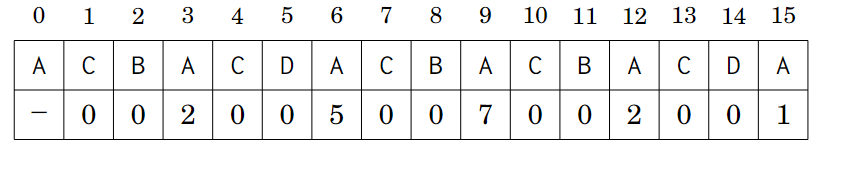
\includegraphics[width=\linewidth]{string_z_algorithm_01.png}
\end{figure}

\begin{lstlisting}
// z_array=length of the longest substring starting from s[i] which is also a prefix of s
vector<int> z_algorithm(const string &s) {
    int n = (int) s.size();
    vector<int> z_array(n);
    int left=0, right=0;
    z_array[0] = 0;
    for(int idx = 1; idx < n; ++idx) {
        z_array[idx] = max(0, min(z_array[idx-left], right-idx+1));
        while (idx+z_array[idx] < n && s[z_array[idx]] == s[idx+z_array[idx]]) {
            left = idx;
            right = idx + z_array[idx];
            z_array[idx]++;
        }
    }
    return z_array;
}
\end{lstlisting}

\subsection{Aho Corasick}
\begin{lstlisting}
// El trie (o prefix tree) guarda un diccionario de strings como un arbol enraizado.
// Aho corasick permite encontrar las ocurrencias de todos los strings del trie en un string s.

const int alpha = 26; // cantidad de letras del lenguaje
const char L = 'a'; // primera letra del lenguaje

struct node {
    int next[alpha], end;
    int link, exit, cnt;
    int& operator[](int i) { return next[i]; }
};

vector<node> trie = {node()};

void add_str(string &s, int id = 1) {
    int u = 0;
    for (auto ch : s) {
        int c = ch-L;
        if (!trie[u][c]) {
            trie[u][c] = trie.size();
            trie.push_back(node());
        }
        u = trie[u][c];
    }
    trie[u].end = id; //con id > 0
    trie[u].cnt++;
}

// aho corasick
void build_ac() {
    queue<int> q; q.push(0);
    while (q.size()) {
        int u = q.front(); q.pop();
        for (int c = 0; c < alpha; ++c) {
            int v = trie[u][c];
            if (!v) trie[u][c] = trie[trie[u].link][c];
            else q.push(v);
            if (!u || !v) continue;
            trie[v].link = trie[trie[u].link][c];
			trie[v].exit = trie[trie[v].link].end ? trie[v].link : trie[trie[v].link].exit;
            trie[v].cnt += trie[trie[v].link].cnt;
        }
    }
}

vector<int> cnt; //cantidad de ocurrencias en s para cada patron

void run_ac(string &s) {
    int u = 0, sz = s.size();
    for (int i = 0; i < sz; ++i) {
        int c = s[i]-L;
        while (u && !trie[u][c]) u = trie[u].link;
        u = trie[u][c];
        int x = u;
        while (x) {
            int id = trie[x].end;
            if (id) cnt[id-1]++;
            x = trie[x].exit;
        }
    }
}
\end{lstlisting}


% MATH
\section{Math}

\subsection{Diophantine}
\begin{lstlisting}
// Use extgcd
template<typename T>
bool diophantine(T a, T b, T c, T & x, T & y, T & g) {
    if (a == 0 && b == 0) {
        if (c == 0) {
            x = y = g = 0;
            return true;
        }
        return false;
    }
    auto [g1, x1, y1] = extgcd(a, b);
    if (c % g1 != 0)
        return false;
    g = g1;
    x = x1 * (c / g);
    y = y1 * (c / g);
    return true;
}
// Usage
// int x, y, g;
// bool can = diophantine(a, b, c, x, y, g);

// a*x + b*y = c -> If and only if gcd(a, b) is a divisor of c
\end{lstlisting}

\subsection{Divisors}
\begin{lstlisting}
template<typename T>
vector<T> divisors(T number) {
    vector<T> ans;
    for (T i = 1; i*i <= number; ++i) {
        if (number % i == 0) {
            if (number/i == i) {
                // if i*i == number
                ans.push_back(i);
            } else {
                // x=i, y=number/i, if x*y==number
                ans.push_back(i);
                ans.push_back(number/i);
            }
        }
    }
    return ans;
}
\end{lstlisting}

\subsection{Ext GCD}
\begin{lstlisting}
template<typename T>
tuple<T, T, T> extgcd(T a, T b) {
    if (a == 0)
        return {b, 0, 1};
    T p = b / a;
    auto [g, y, x] = extgcd(b - p * a, a);
    x -= p * y;
    return {g, x, y};
}
// Usage:
//   auto [g, x, y] = extgcd(a, b);
// = Congruente
// a*x = 1 (mod m) -> If and only if gcd(a, m) == 1
// a*x + m*y = 1

// auto [g, x, y] = extgcd(a, m);

// a*x + b*y = gcd(a, b) 
\end{lstlisting}

\subsection{GCD}
\begin{lstlisting}
template<class T>
T gcd(T a, T b) {
    return (b == 0)?a:gcd(b, a % b);
}
\end{lstlisting}

\subsection{LCM}
\begin{lstlisting}
template<class T>
T lcm(T a, T b) {  
    return (a*b)/gcd<T>(a, b);  
}
\end{lstlisting}

\subsection{Matrix}
\begin{lstlisting}
// Estructura para realizar operaciones de multiplicacion y exponenciacion modular sobre matrices.

const int mod = 1e9+7;

struct matrix {
    vector<vector<int>> v;
    int n, m;
    
    matrix(int n, int m, bool o = false) : n(n), m(m), v(n, vector<int>(m)) {
        if (o) while (n--) v[n][n] = 1;
    }

    matrix operator * (const matrix &o) {
        matrix ans(n, o.m);
        for (int i = 0; i < n; i++)
            for (int k = 0; k < m; k++) if (v[i][k])
                for (int j = 0; j < o.m; j++)
                    ans[i][j] = (1ll*v[i][k]*o.v[k][j] + ans[i][j]) % mod;
        return ans;
    }
    
    vector<int>& operator[] (int i) { return v[i]; }
};

matrix pow(matrix b, ll e) {
    matrix ans(b.n, b.m, true);
    while (e) {
        if (e&1) ans = ans*b;
        b = b*b;
        e /= 2;
    }
    return ans;
}
\end{lstlisting}

\subsection{Lineal Recurrences}
\begin{lstlisting}
// Calcula el n-esimo termino de una recurrencia lineal (que depende de los k terminos anteriores).
// * Llamar init(k) en el main una unica vez si no es necesario inicializar las matrices multiples veces.
// Este ejemplo calcula el fibonacci de n como la suma de los k terminos anteriores de la secuencia (En la secuencia comun k es 2).
// Agregar Matrix Multiplication con un construcctor vacio.

matrix F, T;

void init(int k) {
    F = {k, 1}; // primeros k terminos
    F[k-1][0] = 1;
    T = {k, k}; // fila k-1 = coeficientes: [c_k, c_k-1, ..., c_1]
    for (int i = 0; i < k-1; i++) T[i][i+1] = 1;
    for (int i = 0; i < k; i++) T[k-1][i] = 1;
}

/// O(k^3 log(n))
int fib(ll n, int k = 2) {
    init(k);
    matrix ans = pow(T, n+k-1) * F;
    return ans[0][0];
}
\end{lstlisting}

\subsection{Phi Euler}
\begin{lstlisting}
template<typename T>
T phi_euler(T number) {
    T result = number;
    for(T i = static_cast<T>(2); i*i <= number; ++i) {
        if(number % i != 0)
            continue;
        while(number % i == 0) {
            number /= i;
        }
        result -= result / i;
    }
    if(number > 1)
        result -= result / number;
    return result;
}
\end{lstlisting}

\subsection{Primality Test}
\begin{lstlisting}
template<typename T>
bool is_prime(T number) {
    if(number <= 1)
        return false;
    else if(number <= 3)
        return true;
    if(number%2==0 || number%3==0)
        return false;
    for(T i = 5; i*i <= number; i += 6) {
        if(number%i==0 || number%(i+2)==0)
            return false;
    }
    return true;
    // Time Complexity: O(sqrt(N)), Space Complexity:  O(1)
}
\end{lstlisting}

\subsection{Prime Factos}
\begin{lstlisting}
template<class T>
map<T, int> prime_factors(T number)  {
    map<T, int> factors;
    while (number % 2 == 0) {
        factors[2]++;
        number = number / 2;
    }
    for (T i = 3; i*i <= number; i += 2) {
        while (number % i == 0) {
            factors[i]++;
            number = number / i; 
        }
    }
    if (number > 2)
        factors[number]++;
    return factors;
}
//   for n=100, { 2: 2, 5: 2}
//   2*2*5*5 = 2^2 * 5^2 = 100
\end{lstlisting}

\subsection{Sieve}
\begin{lstlisting}
using int64 = long long;

const int mxN = 1e6;
bool marked[mxN+1];
vector<int> primes;
/// O(mxN log(log(mxN)))
void sieve() {
    marked[0] = marked[1] = true;
    for (int i = 2; i <= mxN; i++) {
        if (marked[i]) continue;
        primes.push_back(i);
        for (int64 j = 1LL * i*i; j <= mxN; j += i)
            marked[j] = true;
    }
}
\end{lstlisting}

\end{document}